In this section the individual components will be discussed in terms of the needed high level sub-parts and their functioning, as well as how those sub-elements interface with one another within the overlaying component and which of them is in charge of interfacing with other components.

\subsection{Database}
The database layer must include a DBMS component, in order to manage the insertion, modification, deletion and logging of transactions on data inside the storage memory.

Regardless of the implementation, the DBMS must guarantee the correct functioning of concurrent transactions and the ACID properties; it also must be a relational DBMS, since the application needs in terms of data storage do not require a more complex structure than the simple one provided by the relational data structure.

The data layer must only be accessible through the Application Server via a dedicated interface. With respect to this, the Application Server must provide a persistence unit to handle the dynamic behaviour of all of the persistent application data.

The Database must be tuned during the implementation phase in order to ensure security by granting data access according to the privilege level of the requester. Sensible data such as passwords and personal information must be encrypted properly before being stored. Users must be granted access only upon provision of correct and valid credentials.

The E-R diagram in Figure \ref{er_dg} illustrates a concept of the Database schema.

\begin{figure}[H]
\begin{center}
		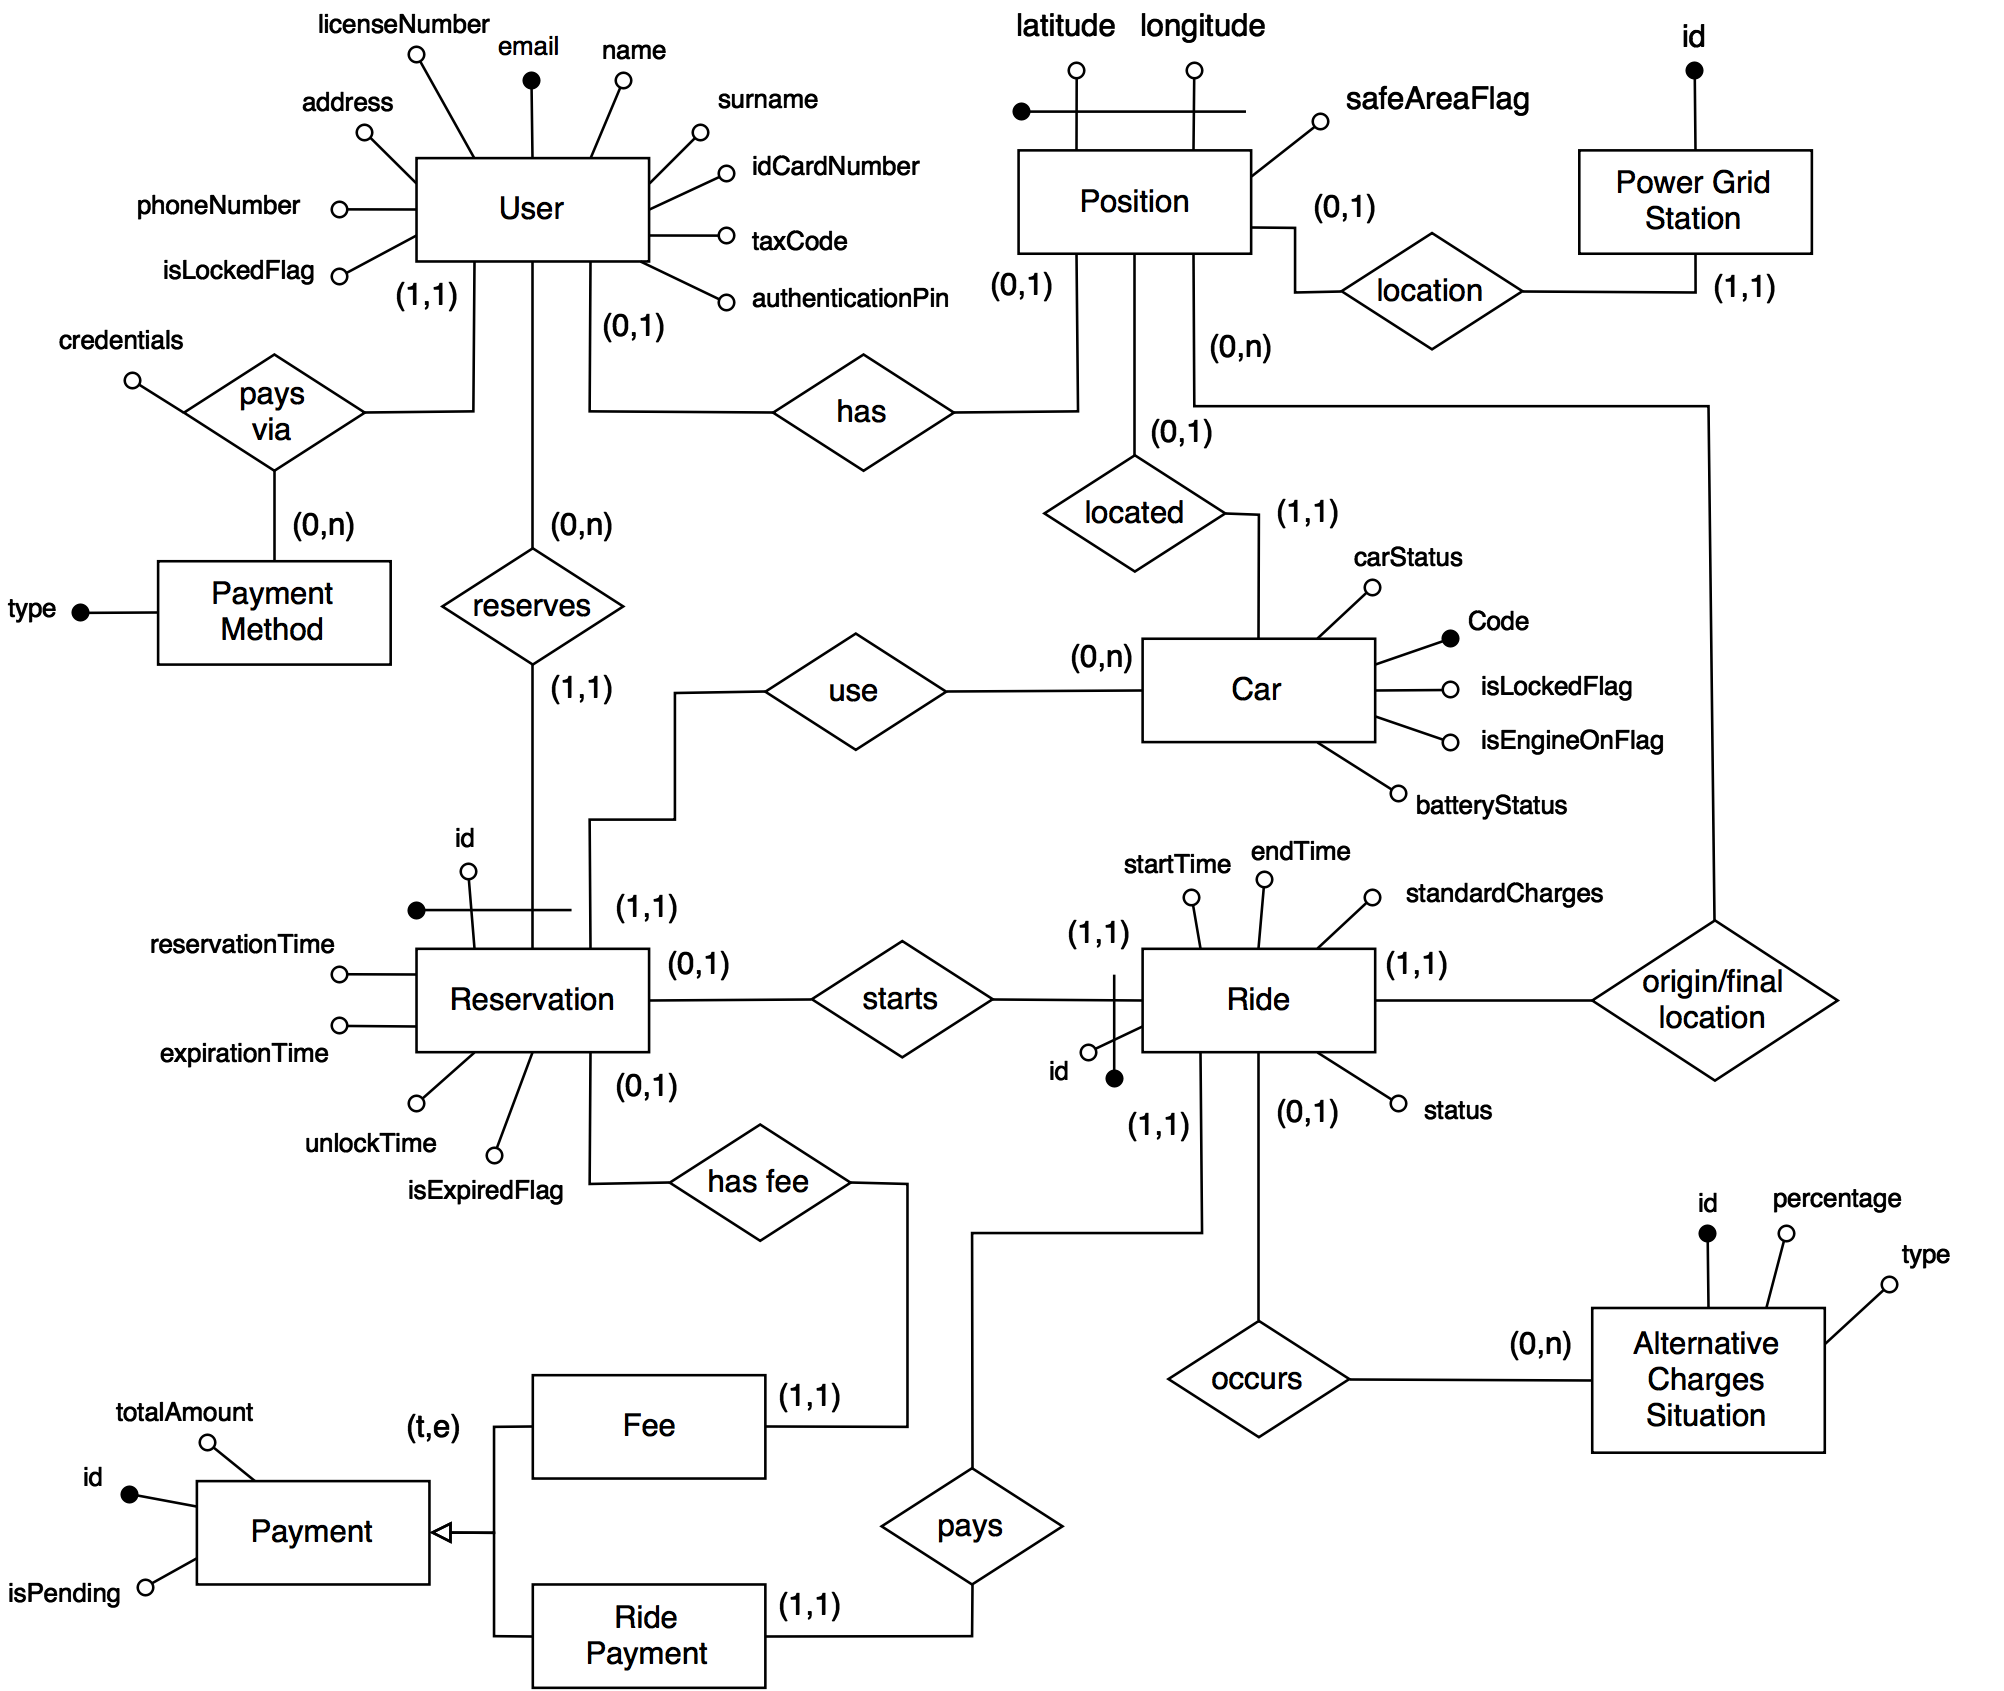
\includegraphics[width=0.9\textwidth]{./arch_design/diagrams/er_dg.png}
		\caption{The E-R diagram of the database schema. Note that the relation named "origin/final location" must be considered as a short-hand notation to indicate two distinct relations: one for the starting location of the ride and one for the ending location.}
		\label{er_dg}
\end{center}
\end{figure}

\subsection{Application Server}
This layer must handle the business logic as a whole and the connections with the data layer and the multiple ways of accessing the application.

The main feature of the Application Server are the specific modules of business logic, which describe business rules and work-flows for each of the functionalities provided by the application itself.

The interface with the data layer must be handled, as stated in the previous section, by a dedicated persistence unit, that will be in charge of the object-relation mapping and dynamic data access and management; this ensures the fact that only the Application Server can access the Database.

The Application Server must provide a means to interface with the Web Server and the mobile and on-board clients via specific APIs in order to decouple the different layers with respect to their individual implementation. Moreover, it must provide a way to communicate with external systems by adapting the application to the existing external infrastructures.

The main business logic modules must include:

\begin{description}
\item[UserManager:] This module will manage all the logic involved with user account management, login, registration, profile customization and management, as well as the generation and provision of user credentials.
\item[ReservationManager:] This module provides the logic behind the reservation management, with particular focus on the timing restrictions, car status updates (via the CarStatusManager) and reservation release conditions. It is also in charge of the controls to be performed in order to avoid multiple reservations by a user; lastly it must handle concurrent reservation issues such as pseudo-simultaneous requests for the same car.
\item[RideManager:] The logic included in this module is in charge of record all useful information about the rides as provided by the on-board application, including ride time, car battery levels and ride charges. It also manages the ride status updates.
\item[MapManager:] This module contains the logic used to locate cars and users, as well as defining the Safe Area boundaries and the power grids locations. It must provide useful data to the ReservationManager and the RideManager logic units, since both of them need localization information to perform their functionalities.
\item[CarStatusManager:] This module includes the logic needed by other components to set the car status of a car. It must also serve as an interface with the external maintenance system by providing an automatic way to signal out-of-service cars.
\item[SecurityAuthenticator:] All the logic in charge of performing user-reservation-car matches is included in this module: this includes the control over cars unlocking and the logic behind the on-board authentication method.
\item[DiscountProvider:] This module is in charge of recording virtuous and bad situations as parameters of rides, so that the PaymentGateway can gather all the needed information to compute the corresponding net total charges.
\item[PaymentGateway:] The logic involved in the computation of final charges is included in this module; moreover, this unit must stand as an interface with the payment handlers upon the act of the automatic payments.
\item[NotificationManager:] Serves as a gateway from all the modules that need to notify the client towards the clients themselves by managing the logic behind the notifications services.
\end{description}

\subsection{Web Server}
The Web Server layer connects clients with the business logic layer in case the access to the application services is performed via web browser.

That being said, it is clear that the main functions to be implemented by this layer will essentially consist of interfaces, since - as stated in Section \ref{high_level_comps} - there will not be any logic implemented within the Web Server besides the presentation of pages.

The presentation must be structured in a clean and simple way, such that the components providing the client with web pages are decoupled as possible from the components that communicates with the business logic subsiding the Application Server in order to fetch relevant data to be shown. The communication must be thought in a way that allows quick and efficient data transfer through textual data files over HTTPS, e.g. XML or JSON.

Adequate APIs must be designed in order to separate in the most efficient way the design of the Web and Application Servers.

\subsection{Mobile Application Client}
The Mobile Client must be designed in a way that makes communications with the Application Server easy and independent from the implementation of both sides. In order to do so, adequate APIs must be defined and used similarly to what has been described for the interactions between the two server layers.

The mobile application UI must be designed following the guidelines provided by the Android and iOS producers.

The application must provide a software module that manages the GPS connection of the device and keeps track of locations data, providing it to the Application Server to be processed.

\subsection{On-Board Application Client}
The On-Board Application consists of an application designed to run on pre-existing embedded devices on every car. The devices come together with the rest of the car equipment directly from the manufacturer. For this reason, the application must be designed following the guidelines provided by the manufacturer and based on given APIs.

The software module to be included in the application must manage the GPS locations of cars and the connection with the car sensors, as well as the transmission of all car-related data to the Application Server for the processing needed by the various business logic functions.

As far as the interface with the Application Server, the same considerations made with respect to the mobile application must be taken into account also for the on-board application.

\begin{figure}[H]
\begin{center}
		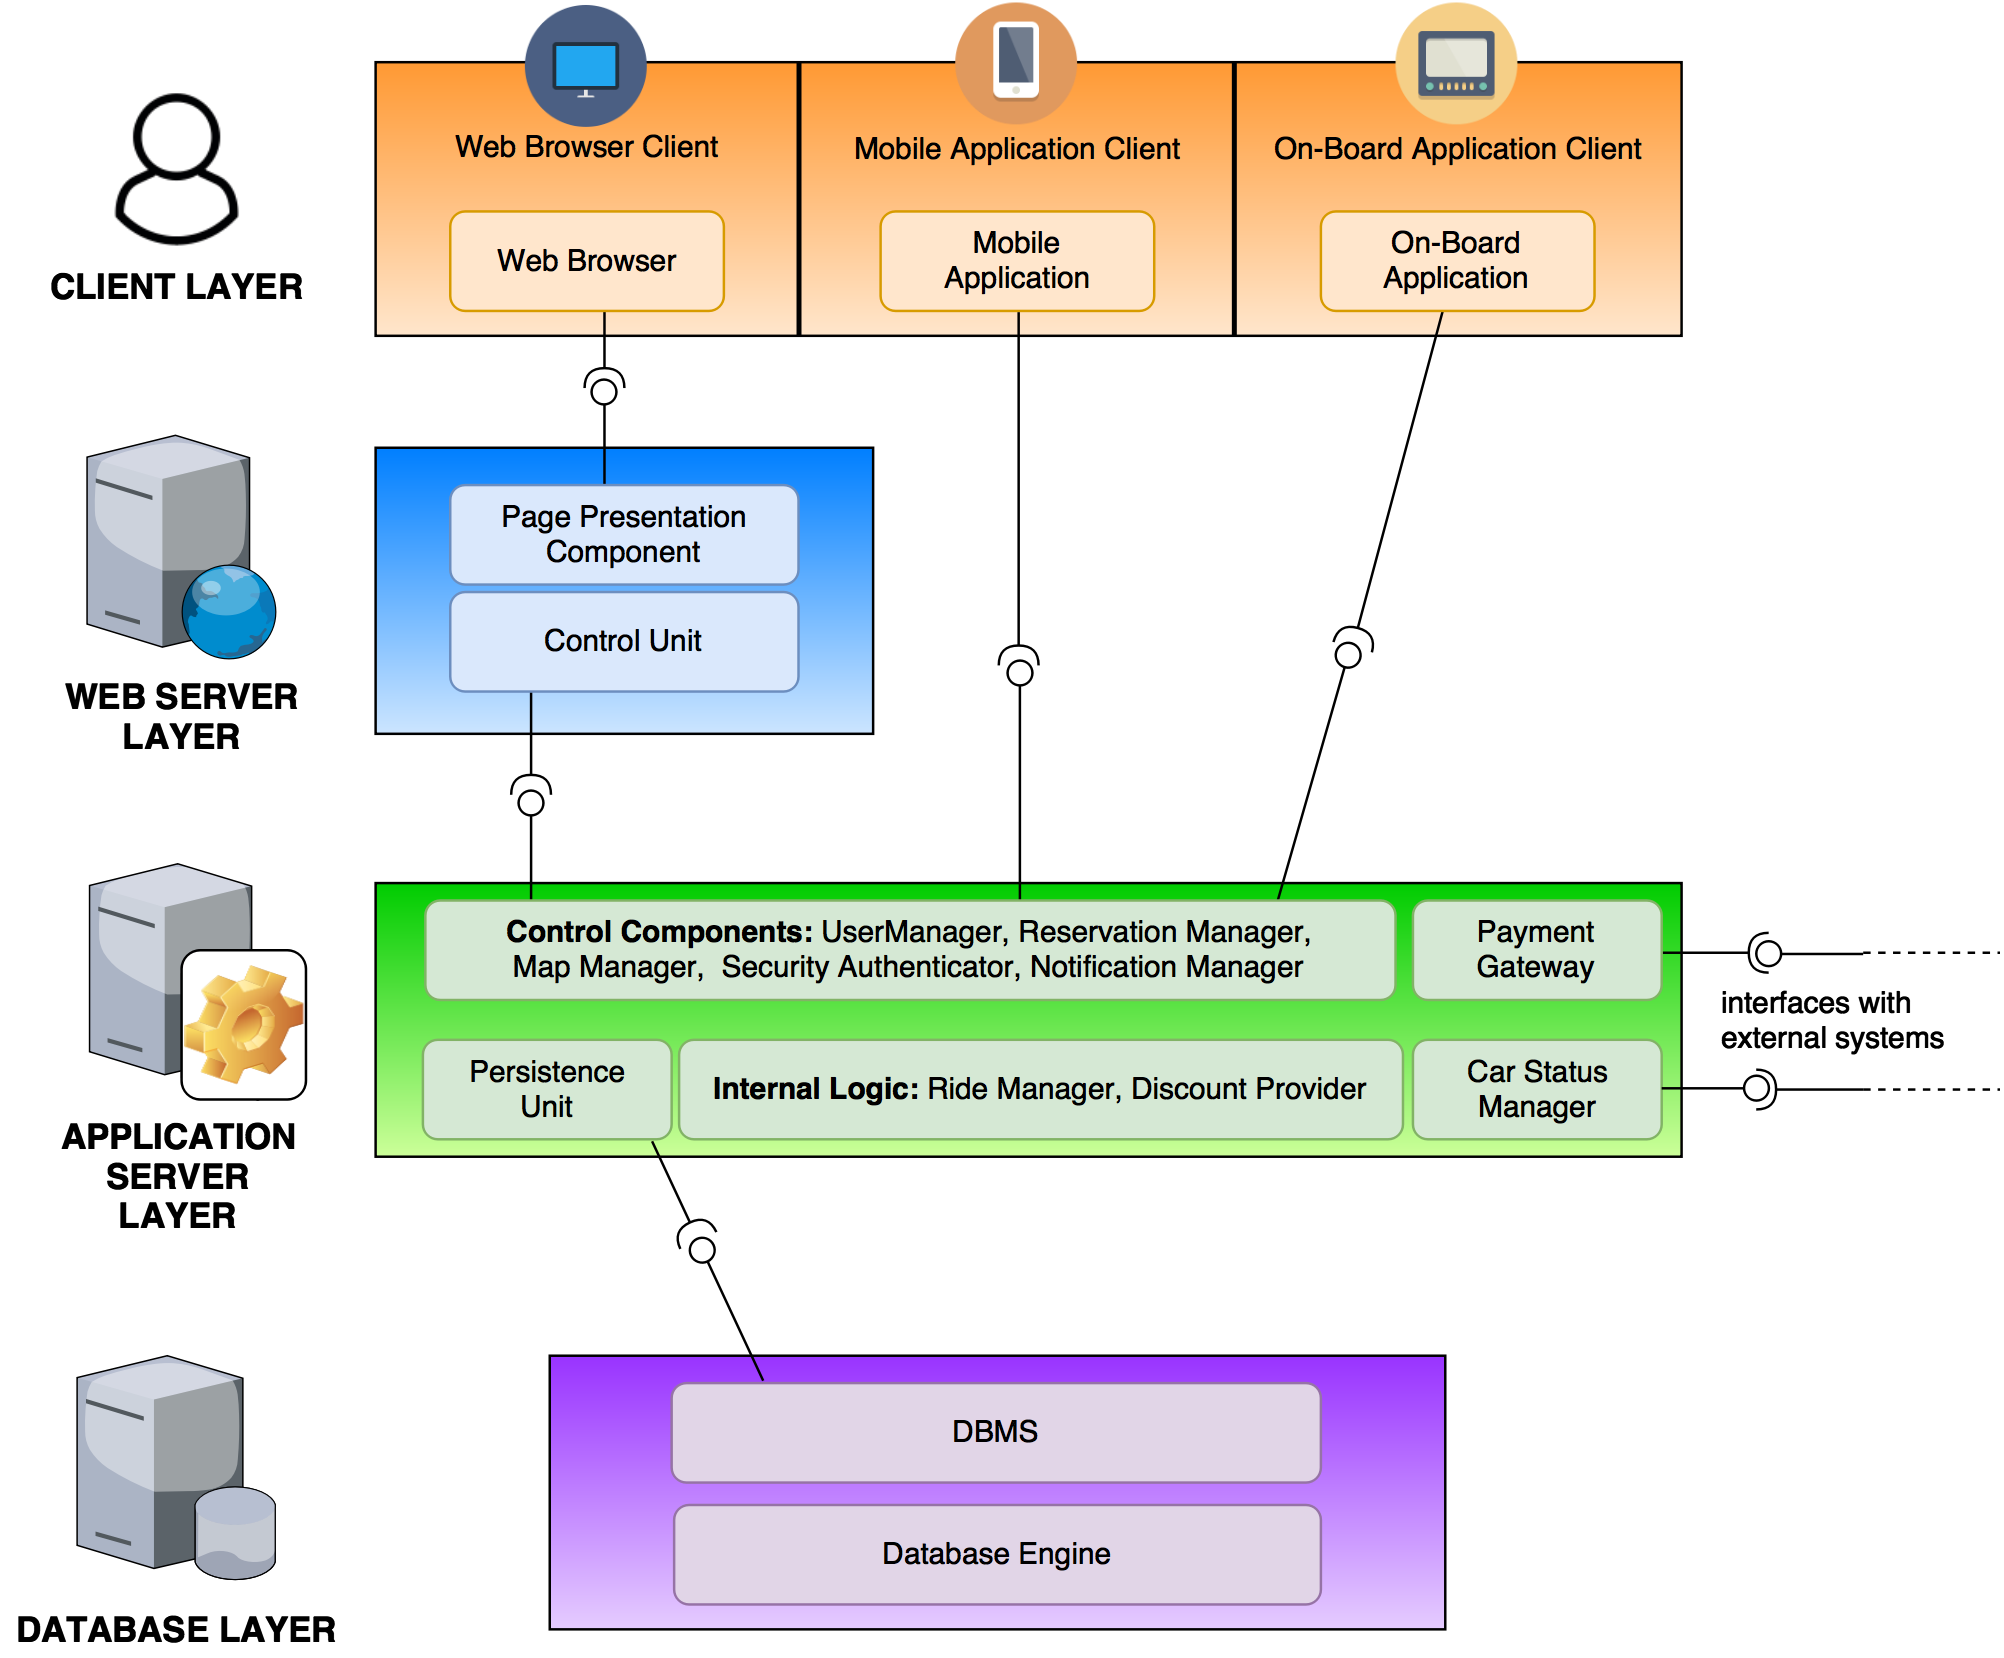
\includegraphics[width=\textwidth]{./arch_design/diagrams/global_comp_view.png}
		\caption{The global component view. Note that in the application server layer, most modules have been collapsed and only those that are relevant to particular interfaces have been highlighted. The modules interacting with the clients are more than one, so the connection has been specified with a macro-module containing all the access points.}
		\label{global_comp_view}
\end{center}
\end{figure}

\subsection{Implementation Choices}
\subsubsection{Database Implementation}
The implementation choices for the Database layer are the following:
\begin{itemize}
\item MySQL 5.7 as the relational DBMS;
\item InnoDB as the subsiding database engine; InnoDB is a good choice for this application, because it manages concurrent access to the same tables in a very clean and quick way;
\item The Java Persistence API (JPA) within the Application Server will serve as an interface with the Database.
\end{itemize}

\subsubsection{Application Server Implementation}
The main choice for this layer is the use of Java Enterprise Edition 7 (JEE). This was the most reasonable option for several reasons: the final product is a large-scope application, and thus needs distribution to great numbers of clients simultaneously; for the same reason, it needs to satisfy continuously evolving functional requirements and customer demands; JEE also allows the developers to focus on the logic behind the main functionalities while being supported by a series of reliable APIs and tools that, among other features, can guarantee the main non-functional requirements of the case (e.g. security, reliability, availability...); lastly, it can reduce the complexity of the application by using mechanisms and models that easily adapt to a large-scale project.

The specific implementation choices are:
\begin{itemize}
\item GlassFish Server as the Application Server implementation;
\item Enterprise JavaBeans (EJB) to implement the single business logic modules described in the sections above. These will be appropriately subdivided into EJB containers as specified by the JEE documentation;
\item Java Persistence API (JPA) as the persitence unit to perform the object-relation mapping and the Database access. JPA Entities will be used to implement the object representation of the data entities;
\item JAX-RS to implement proper RESTful APIs to interface with clients and the Web Server;
\item To interface with external systems, existing RESTful APIs defined by the partner (payment handlers, maintenance system) will be used.
\end{itemize}

\begin{figure}[H]
\begin{center}
		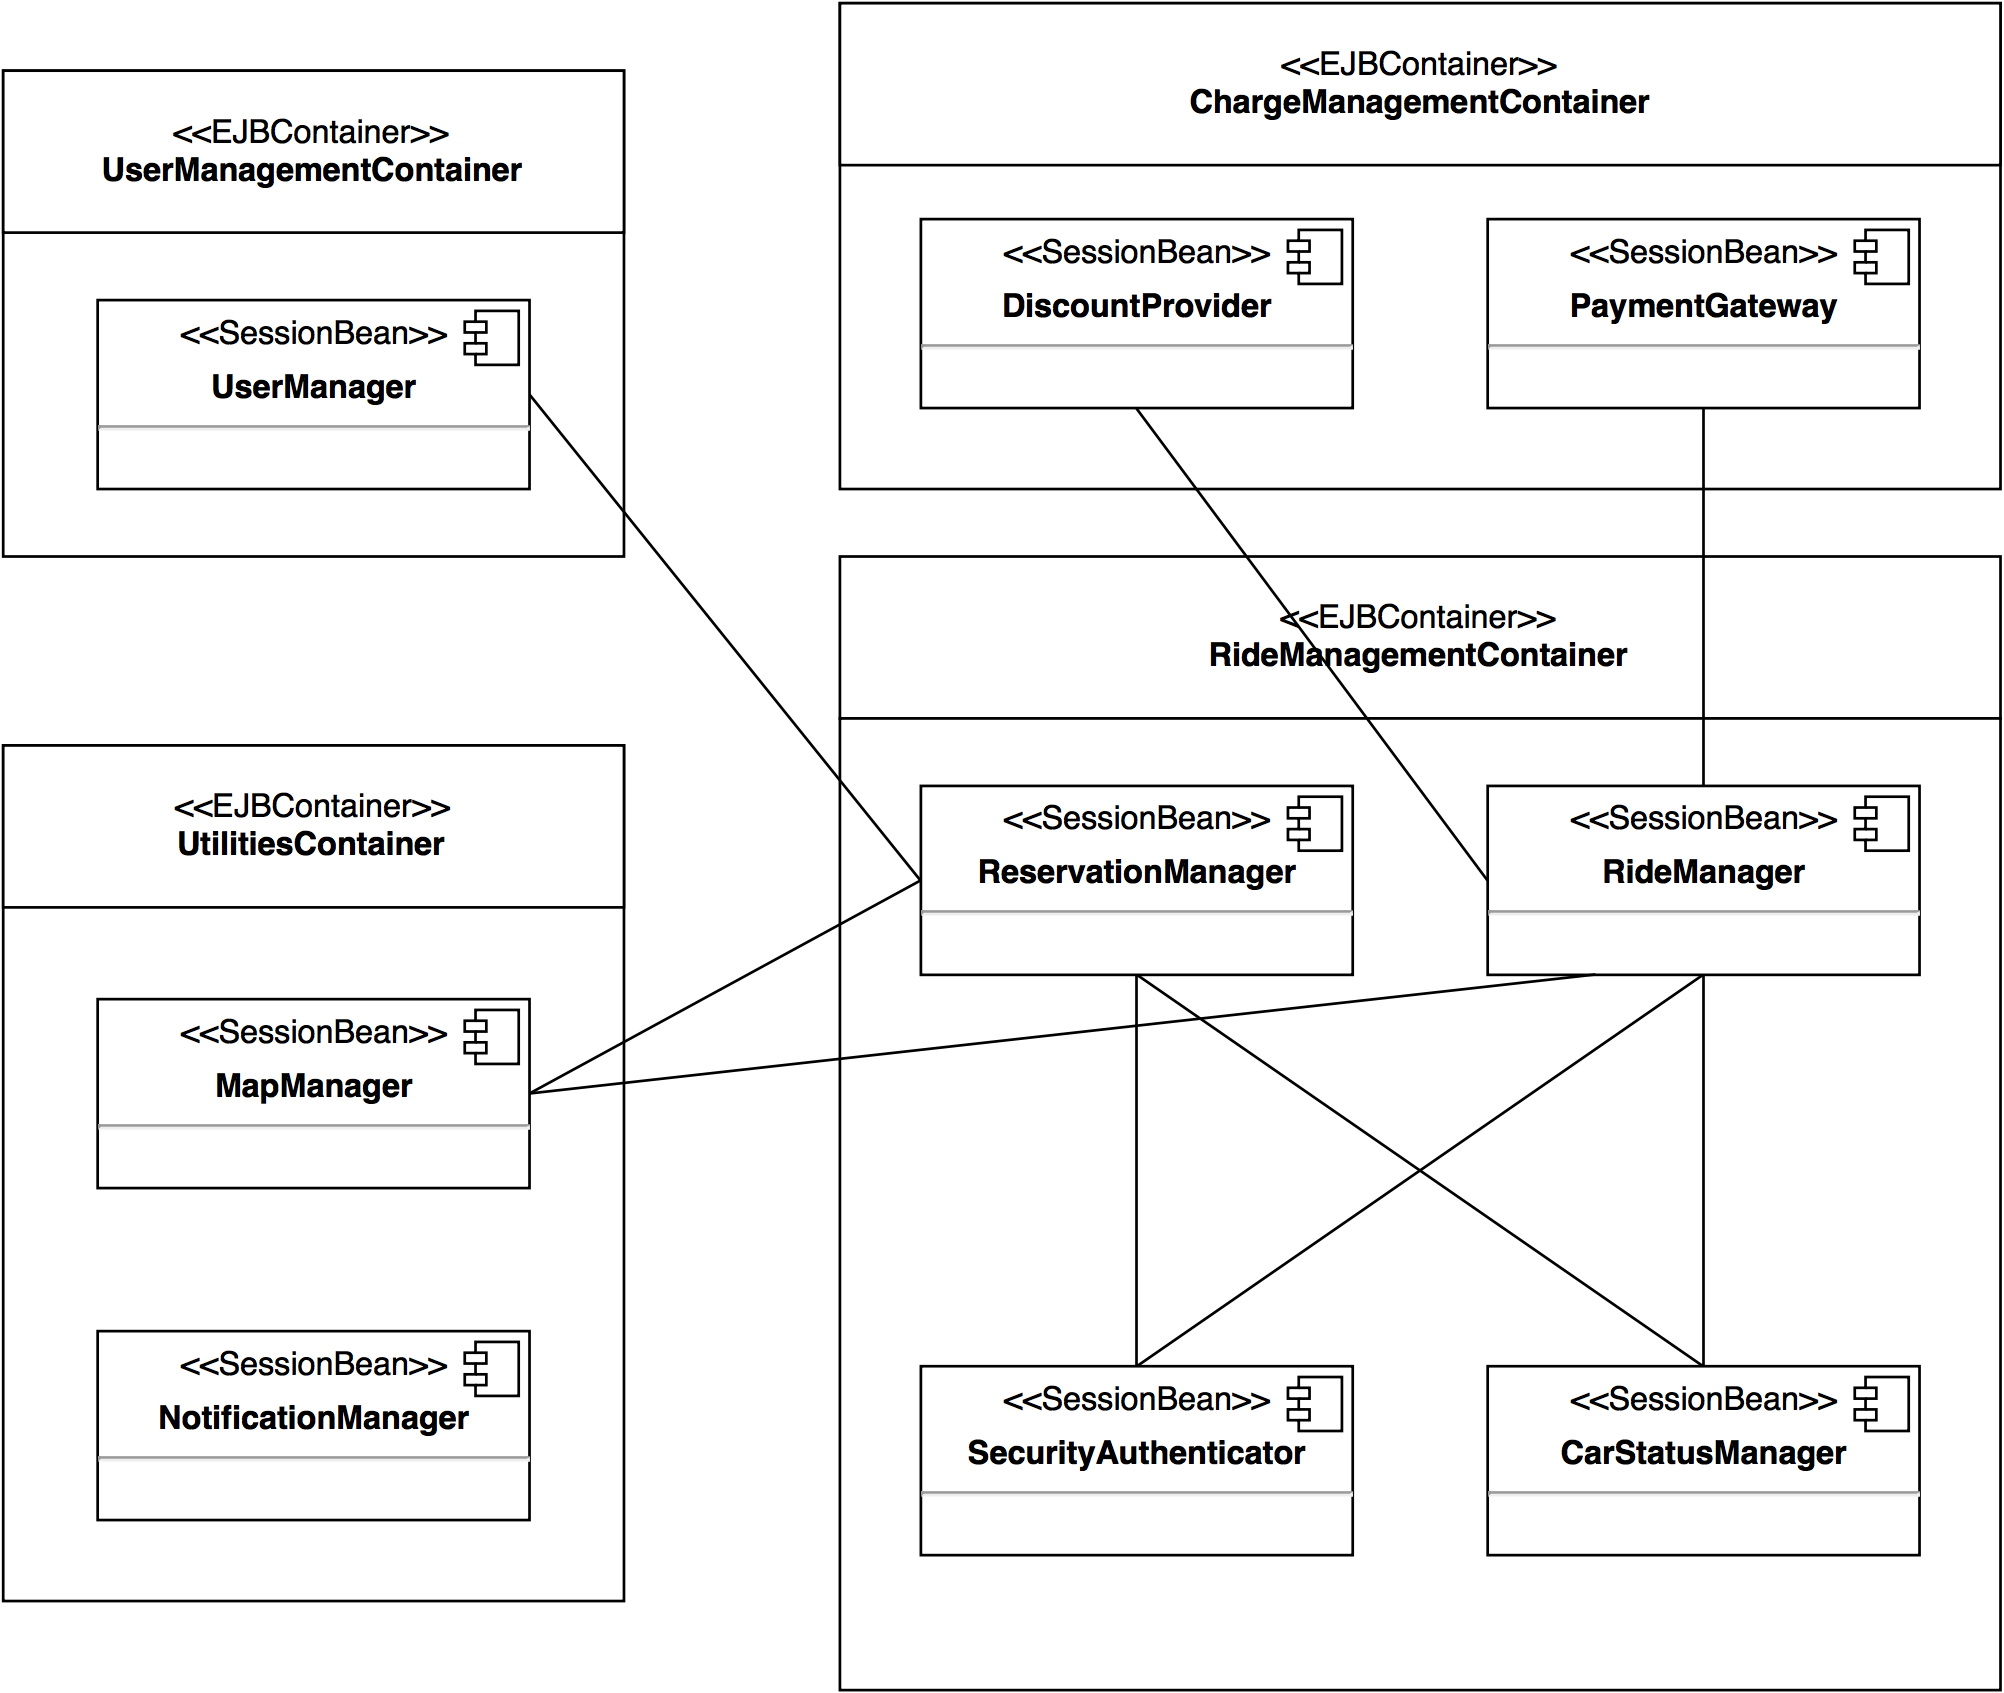
\includegraphics[width=\textwidth]{./arch_design/diagrams/app_server_comps.png}
		\caption{The components of the application server implemented as session beans to develop the business logic.}
		\label{app_server_comps}
\end{center}
\end{figure}

\subsubsection{Web Server Implementation}
Based on the choices made for the Application Server implementation, an easy way to avoid interface issues between the two server layers is to use the GlassFish functionalities for the Web Server as well.

This layer will also heavily rely on JEE: the core components of the Web Server will be implemented with JEE web components. In particular, the application will use JavaServer Pages (JSP) as the technology for developing the web presentation logic based on the MVC pattern. The choice of JEE also allows the Web Server to make use of Servlets to manage specific interactions when necessary.

The interface with the Application Server will be provided by the same RESTful API specified in the previous subsection.

\begin{figure}[H]
\begin{center}
		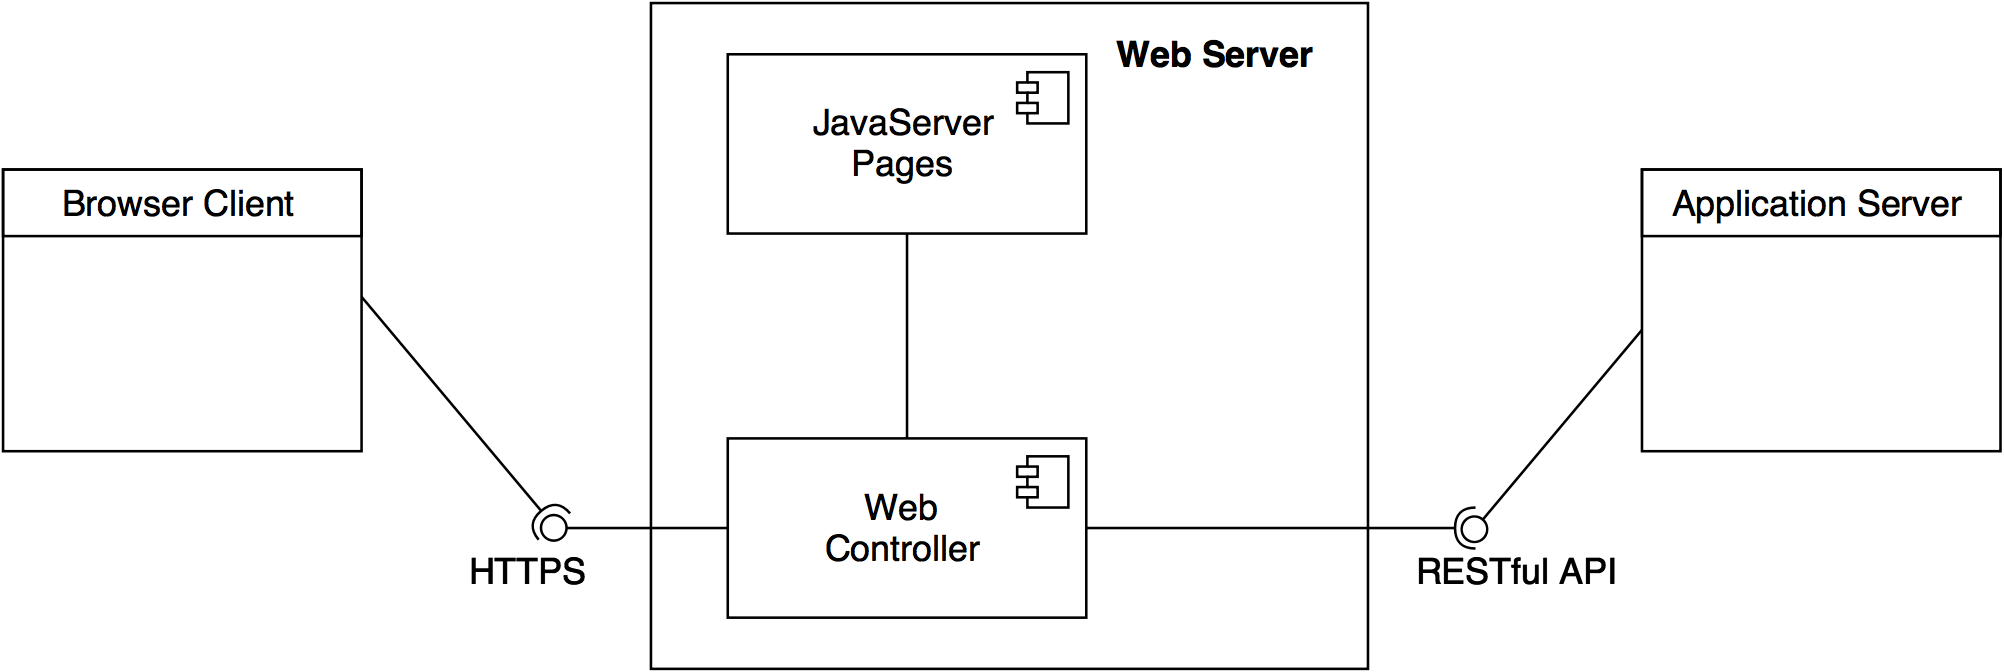
\includegraphics[width=\textwidth]{./arch_design/diagrams/web_server.png}
		\caption{The components of the web server and their interfaces with other layers.}
		\label{web_server}
\end{center}
\end{figure}

\subsubsection{Mobile Application Client Implementation}
The mobile application UI must be designed following the design guidelines provided by the devices' manufacturers. Two architectures must be supported: iOS and Android. The iOS application must be written in Swift, while the Android one must be implemented in Java.

The core of both application must be a Controller that communicates user inputs (after translating them from the UI input) to the Application Server via RESTful APIs. The access to the GPS of the devices must be performed through the default frameworks of the respective systems.

\begin{figure}[H]
\begin{center}
		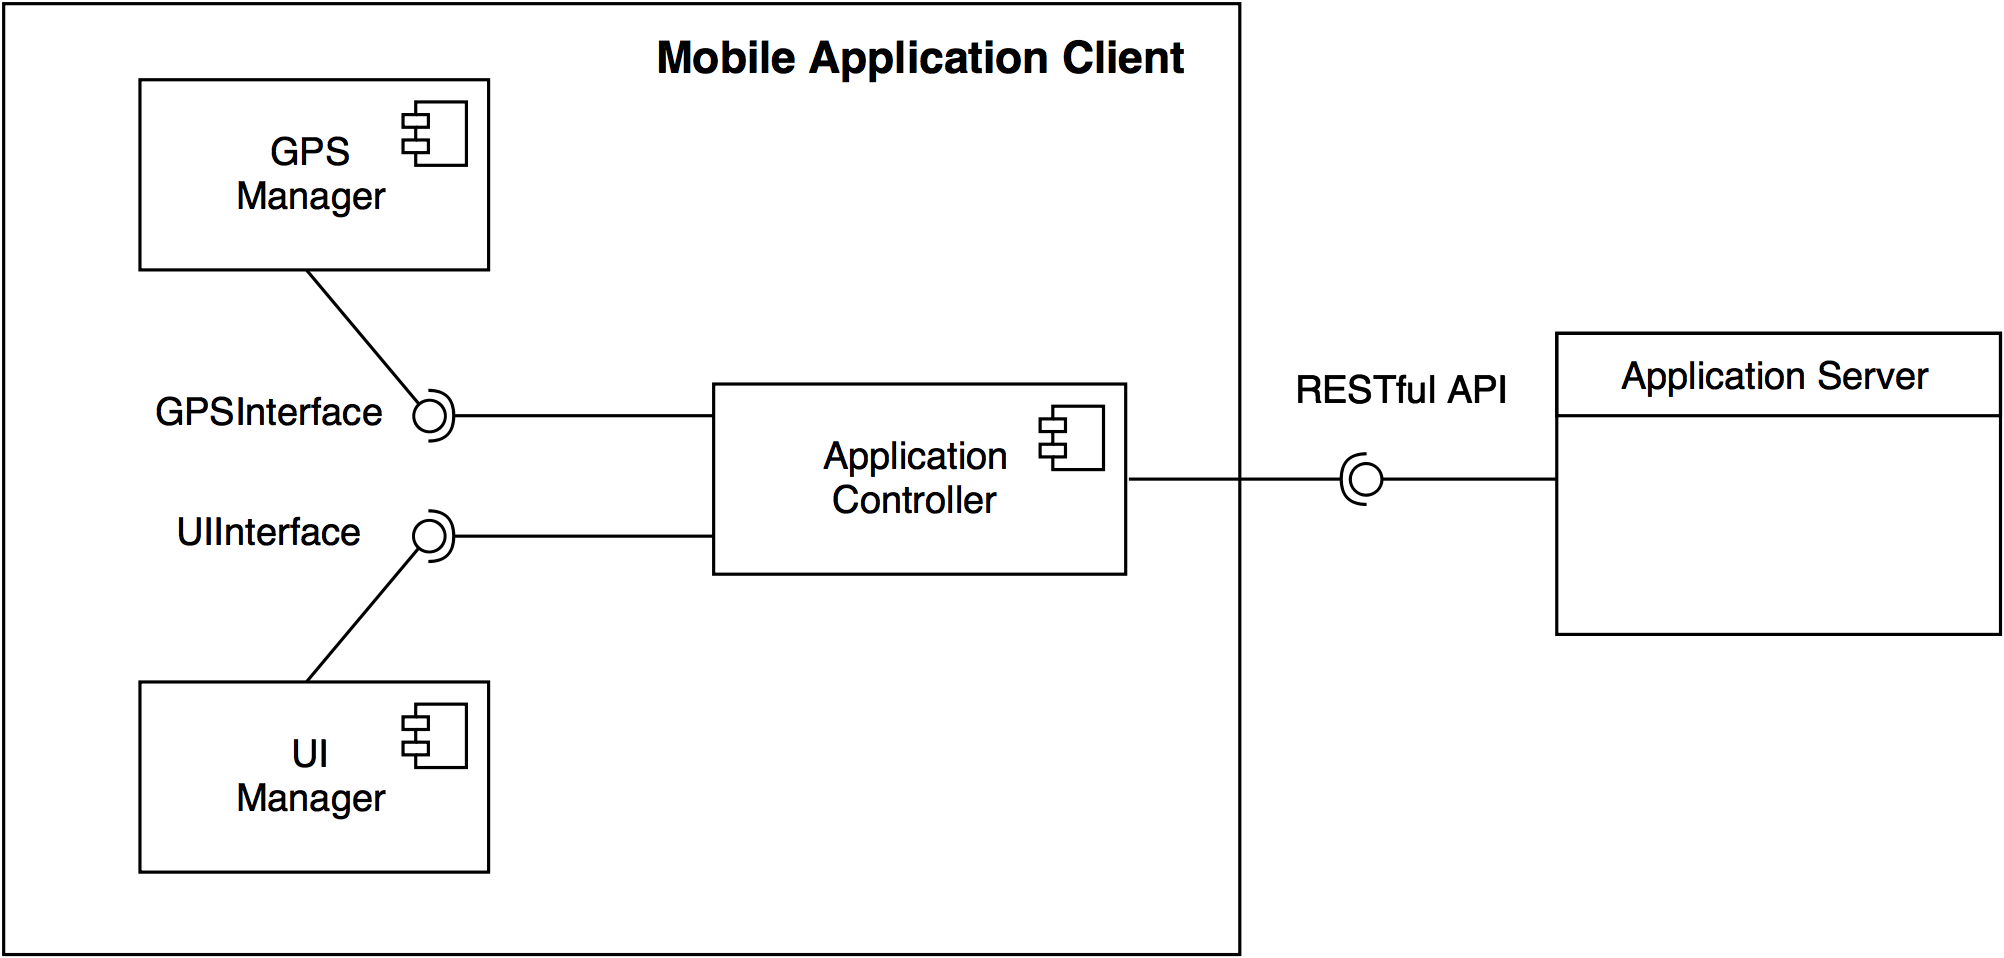
\includegraphics[width=\textwidth]{./arch_design/diagrams/mobile_app_comps.png}
		\caption{The components of the mobile application.}
		\label{mobile_app_comps}
\end{center}
\end{figure}

\subsubsection{On-Board Application Client Implementation}
The on-board application must strictly follow the car manufacturer guidelines for the development. The given APIs must be used to properly connect with the car equipment and sensors via the car CAN bus.

Since the car embedded devices have limited hardware specifications, the software must be written in C/C++. The user interface must be managed by a dedicated unit. The core of the application must include a GPS manager and a mobile connectivity unit. The communication with the Application Server must be performed by the connectivity unit via an adequate RESTful API. Data-flows from the car sensors must be handled by a separated data collection unit and properly evaluated by a data processing unit. The single elements will be coordinated by a Controller.

\begin{figure}[H]
\begin{center}
		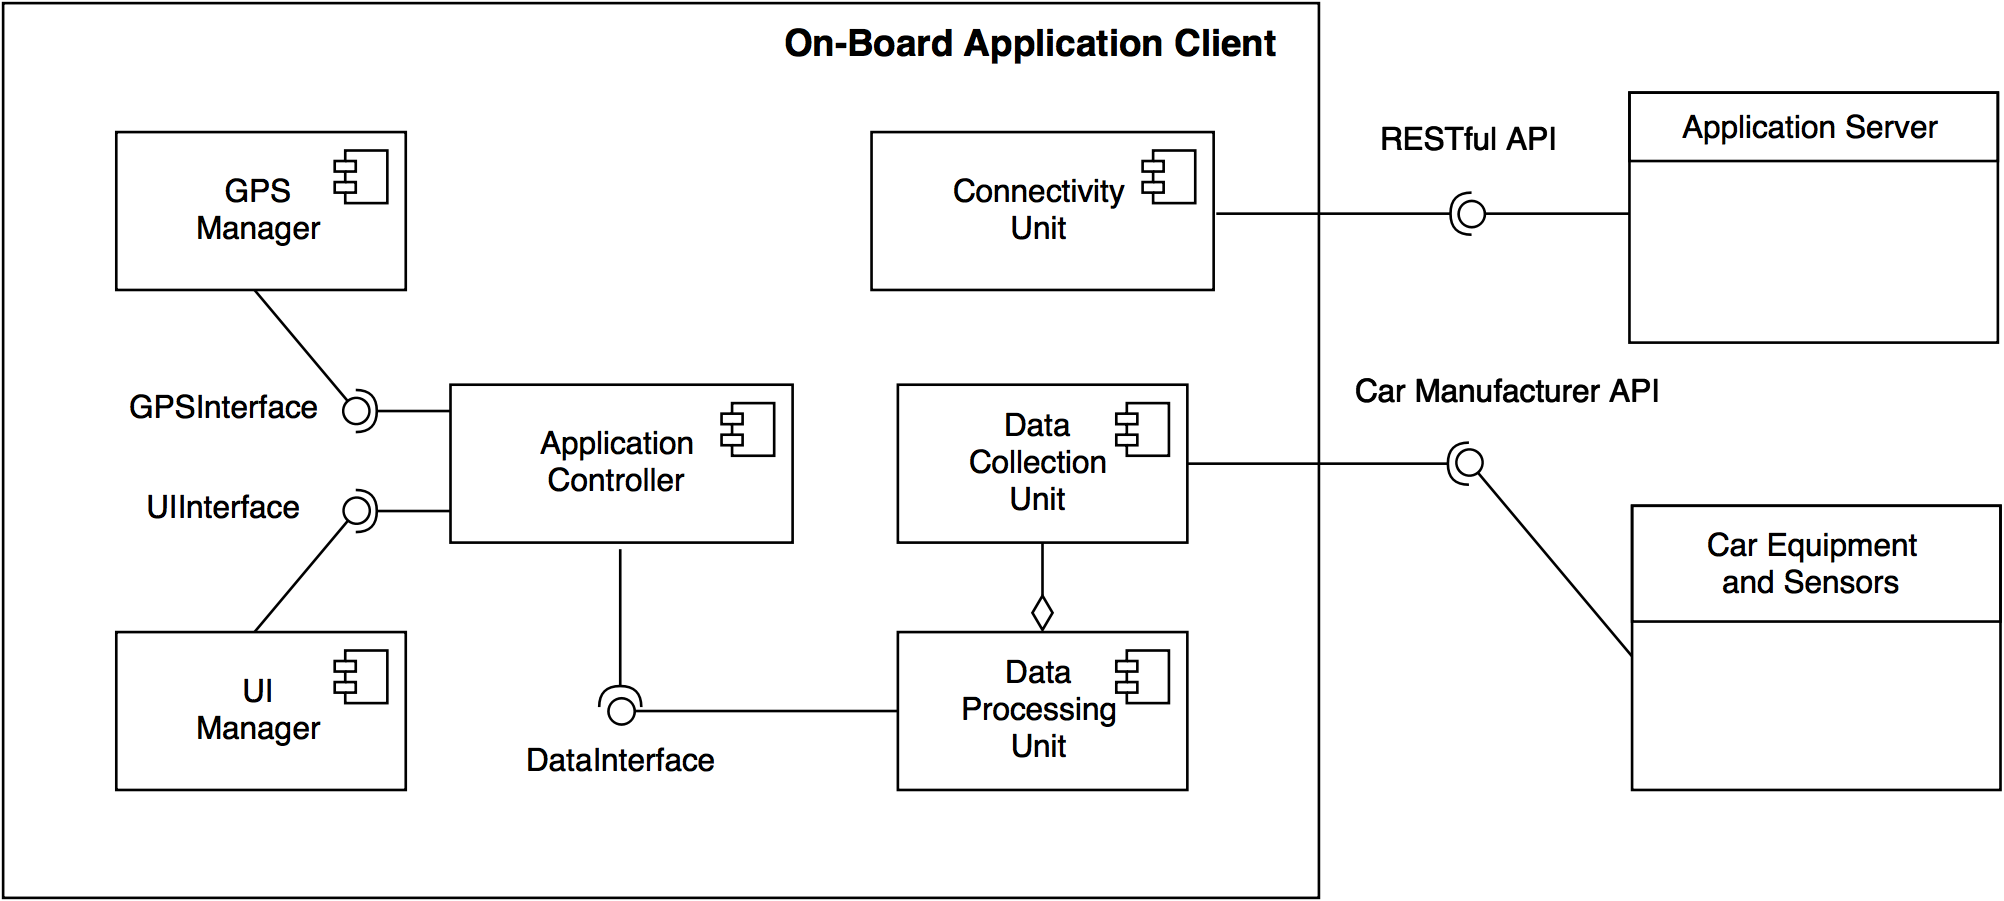
\includegraphics[width=\textwidth]{./arch_design/diagrams/on_board_comps.png}
		\caption{The components of the on-board application.}
		\label{on_board_comps}
\end{center}
\end{figure}

\begin{figure}[H]
\begin{center}
		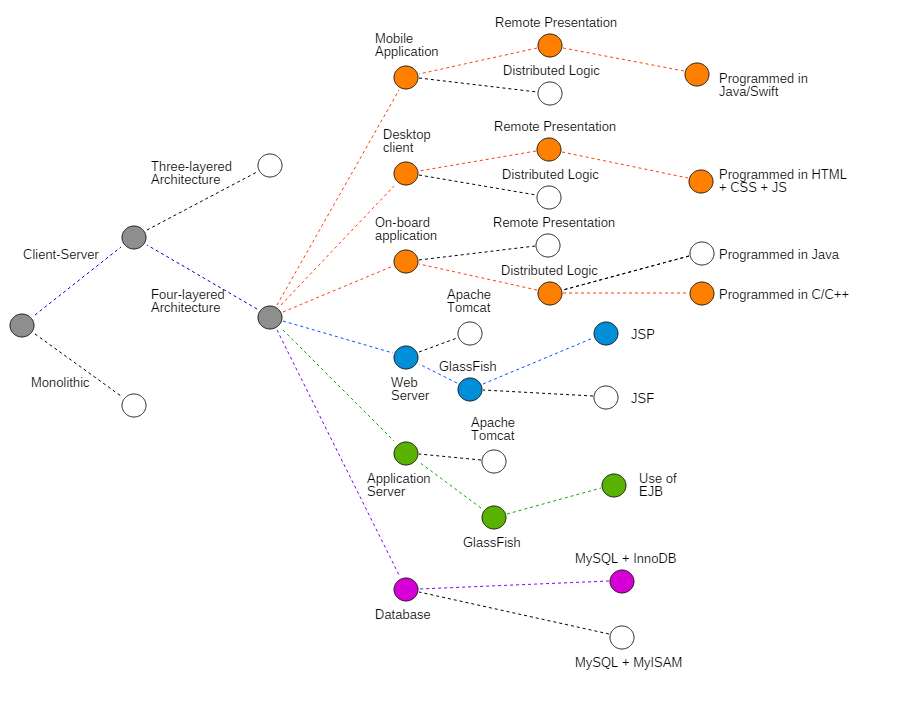
\includegraphics[width=\textwidth]{./arch_design/diagrams/choices_tree.png}
		\caption{The overall decision tree for the first phase of the architectural design.}
		\label{overall_choices}
\end{center}
\end{figure}